% ME3297 - Team project final report, built on the HCMUT report template
% Build: pdflatex -shell-escape report.tex ; bibtex report ; pdflatex -shell-escape report.tex (x2)
% Figures are read directly from ../outputs/figures/ (produced by ../run_all.py).
\documentclass[twoside,final]{hcmut-report}
\usepackage{codespace}

% Encodings
\usepackage{gensymb,textcomp}

% Better tables
\usepackage{array,longtable,multicol,multirow,siunitx,tabularx}

% Better enum
\usepackage{enumitem}

% Graphics
\usepackage{caption,float,subcaption}

% Add options for figures, like max width, framing, etc.
\usepackage[export]{adjustbox}

% References
% Use \Cref{} instead of \ref{}
\usepackage[nameinlink]{cleveref}

% Wider text block and tighter header/footer than the template defaults
\geometry{
  left=2cm, right=2cm, top=0.6cm, bottom=1.2cm,
  includeheadfoot=true,
  headheight=35pt, headsep=16pt, footskip=18pt
}
% fancyhdr fixed the header width before the geometry change; match the new text width
\setlength{\headwidth}{\textwidth}

% Figures produced by the analysis code
\graphicspath{{../outputs/figures/}{graphics/}}

% Configurations
\deptname{School of Industrial Management}
\coursename{\parbox{0.88\linewidth}{\centering ME3297 -- Applications of Artificial Intelligence in Supply Chain Management}}
\reporttype{Major Assignment -- Final Report\\[2pt]\normalsize Section L\_\_ \quad Team \_\_}
\title{Flagging Orders at Risk of Late Delivery\\[4pt]\large DataCo Smart Supply Chain -- a decision at order release}
\advisor{& Ngô Đình Phương &}
\stuname{%
  & Lương Trương Quang Huy & 2352385 \\
  & Lê Tuấn Tài            & 2312997 \\
  & Nguyễn Quốc Đăng Khoa  & 2311625 \\
  & Nguyễn Lê Chí Kiên     & 2352643 \\
  & Phạm Hải Nam           & 2352783 \\
  & Lê Thanh Duy           & 2352178 \\
}

% Set depth of numbering for counters
\AtBeginDocument{\counterwithin{lstlisting}{section}}

\setcounter{tocdepth}{2}

% Compact lists
\setlist{itemsep=1pt,topsep=3pt}

% Custom commands
\newcommand{\tcode}[1]{\texttt{#1}}
\newcommand{\usd}[1]{\$#1}

\begin{document}
\hypersetup{pageanchor=false}  % avoid duplicate page anchors before numbering restarts
\coverpage%

% Cover and table of contents are not numbered; page 1 is the executive summary
\pagenumbering{gobble}
\begin{spacing}{1.0}
\tableofcontents
\end{spacing}

\clearpage
\pagenumbering{arabic}
\hypersetup{pageanchor=true}
\section{Executive summary}
\label{sec:summary}

\textbf{Recommendation.} DataCo's late deliveries are mostly a promise-setting problem, not an
order-selection problem. We recommend three actions.
\begin{enumerate}
  \item \textbf{Change two promises first.} First Class is promised in 1 day but every First Class
        order takes exactly 2 days, so all of them are late. Same Day orders placed after 12:00
        always arrive the next day. Promising 2 days for First Class, and next-day delivery for
        afternoon Same Day orders, cuts late orders from \textbf{246 to 169 per week ($-31\%$)}.
        The average promise lengthens by only 0.18 days.
  \item \textbf{At order release, flag orders with a five-row lookup table, not a
        machine-learning model.} Flag an order when $P(\text{late})\times\text{order value} >
        \usd{200}$. This flags about 187 of 428 orders per week, catches 129 late ones and
        saves about \textbf{\usd{2{,}400} per week}, against \usd{1{,}500} for the best fixed rule.
  \item \textbf{Re-check on real delivery records before deploying.} The delivery timings in this
        dataset follow deterministic, apparently generated patterns.
\end{enumerate}

\textbf{Evidence.} We trained four baselines and six models (decision tree, random forest,
gradient boosting, SVM, MLP and logistic regression) on 49{,}826 orders from 2015--2017-06,
and tested them once on 13{,}071 later orders. The best models, the decision tree (PR-AUC
$0.854 \pm 0.005$ over 5 rolling-origin folds) and gradient boosting ($0.853 \pm 0.003$), tie
with the lookup table ($0.855 \pm 0.002$). Within Second and Standard Class the models rank
orders at chance level (ROC-AUC 0.47--0.52), and across 36 cost scenarios the best model and
the table stay within \usd{25} per week of each other. Shipping mode and order hour carry the
entire signal.

\section{Problem and decision}
\label{sec:problem}

\subsection{Supply-chain situation}
DataCo Global sells clothing, sporting goods and electronics online to 164 countries. At
checkout the customer chooses a shipping mode, and each mode carries a fixed promise: Same Day
(0 days), First Class (1), Second Class (2) or Standard Class (4). In the data, 57\% of the
orders that were not cancelled arrived late. Each late order costs goodwill credits, repeat
contacts and, eventually, customers.

\subsection{Decision, decision-maker and moment}
\begin{itemize}
  \item \textbf{Decision.} Should this order be treated as high-risk before it leaves the
        warehouse? If so, it gets priority handling or a mode upgrade, or customer service
        contacts the buyer in advance with a realistic date.
  \item \textbf{Decision-maker.} The fulfilment planner, with customer service acting on the
        flagged list.
  \item \textbf{Moment.} Order release: the order has been placed and paid, but not yet
        dispatched. At that moment the planner knows the order contents, prices and discounts,
        the customer and destination, the chosen mode and its promise, and the time of day. The
        planner does \emph{not} know the actual transit time or the final order status.
\end{itemize}

\subsection{Target and what is known at the moment of decision}
The target is \tcode{Late\_delivery\_risk} (1 = late). We verified that for every order that was
not cancelled it equals \tcode{Days for shipping (real)} $>$ \tcode{Days for shipment
(scheduled)}. Actual transit takes 0--6 days, and we assume the outcome is recorded one day after delivery,
so the label becomes known 1--7 days after the order. \Cref{sec:prep} lists the
columns we excluded because they are only known after the outcome.

\subsection{Baselines the models must beat}
The dataset does not describe DataCo's current practice, so we built baselines of increasing
strength:
\begin{enumerate}
  \item \textbf{Majority class}: treat every order as late (57\% of orders are late).
  \item \textbf{Rule A}, our proxy for current practice: flag every First and Second Class
        order, because these modes carry the tightest promises.
  \item \textbf{Rule B}: Rule A, plus Same Day orders placed at or after a cut-off hour learned
        from the training data.
  \item \textbf{Lookup table}: the historical late share for each mode, with Same Day split at
        the cut-off hour. This uses the same information as Rule B but outputs a probability.
\end{enumerate}
A model only adds value if it beats the lookup table.

\subsection{Cost of each kind of error}
\label{subsec:costs}
We assume the following costs (\Cref{tab:costs}). The dataset contains none of them, so
\Cref{sec:recommendation} tests 36 alternative combinations.

\begin{table}[!htbp]
  \centering
  \caption{Cost assumptions per order (USD). $v$ is the order value; the median is about \usd{560} in the training period.}
  \label{tab:costs}
  \small
  \begin{tabularx}{\linewidth}{l c X}
    \toprule
    \textbf{Outcome} & \textbf{Cost} & \textbf{Reasoning} \\
    \midrule
    False alarm (flagged, on time)  & \usd{10}                    & priority handling, an upgrade or a call that was not needed \\
    Missed late order               & $0.10\,v$ ($\approx\usd{56}$) & goodwill credit, repeat contacts, churn risk \\
    Caught late order               & $\usd{10} + 0.05\,v$         & action cost; half of the late-delivery cost is avoided \\
    Correctly not flagged           & 0                           & -- \\
    \bottomrule
  \end{tabularx}
\end{table}

At the median order value, a missed late order costs about five times as much as a false
alarm. For cheap orders the ratio falls below one, which drives the policy in
\Cref{sec:recommendation}.

\section{Data}
\label{sec:data}

\subsection{Source and licence}
We use \emph{DataCo Smart Supply Chain for Big Data Analysis}, Version 5, by Constante, Silva
and Pereira\cite{dataco2019} (Route A, approved dataset no.~1). It is published on Mendeley Data
under a CC BY 4.0 licence and cited as the publisher requires. We use only the main table,
\tcode{DataCoSupplyChainDataset.csv}, and its column description file. The clickstream log in the
same archive is not used.

\subsection{Structure and size}
The file holds \textbf{180{,}519 order lines $\times$ 53 columns}: 65{,}752 orders (2.7 lines
each on average) from 20{,}652 customers, covering 118 products, placed between 2015-01-01 and
2018-01-31. Every line of an order carries the same label and the same order-level attributes
(the pipeline checks this), so we model at the \emph{order} level, where the decision is taken. After removing 7{,}754 cancelled
lines (\Cref{sec:prep}), \textbf{62{,}897 orders} remain. \Cref{app:dictionary} gives the data
dictionary for all 28 features used.

\subsection{Quality assessment}
\begin{itemize}
  \item \textbf{Missing values} are rare, and only in columns we do not use:
        \tcode{Product Description} is 100\% empty, \tcode{Order Zipcode} is 86.2\% empty,
        \tcode{Customer Lname} is missing in 8 rows and \tcode{Customer Zipcode} in 3. No feature
        we use has a missing value.
  \item \textbf{Outliers} were counted with the $1.5\times$IQR rule. We kept them, because
        expensive orders and heavy losses are real business events. Flagged values:
        line \tcode{Sales} 0.3\%, product price 1.1\%, and \tcode{Benefit per order} 10.5\%
        (range $-\usd{4{,}275}$ to $+\usd{912}$).
  \item \textbf{Class balance and concentration.} 57.3\% of orders are late, so predicting
        ``late'' for every order already scores 57\% accuracy. By mode (\Cref{fig:mode}): First
        Class 100\%, Second 80\%, Same Day 48\%, Standard 40\%.
  \item \textbf{Drift.} From 2017-Q4, orders shrink from about 3.0 lines to 1.0 line and the
        active catalogue falls from about 55 to 10 products. The median order value drops from
        about \usd{600} to \usd{85} (2018-Q1). Order counts and the late share stay stable
        (\Cref{fig:monthly}).
\end{itemize}

\begin{figure}[!htbp]
  \centering
  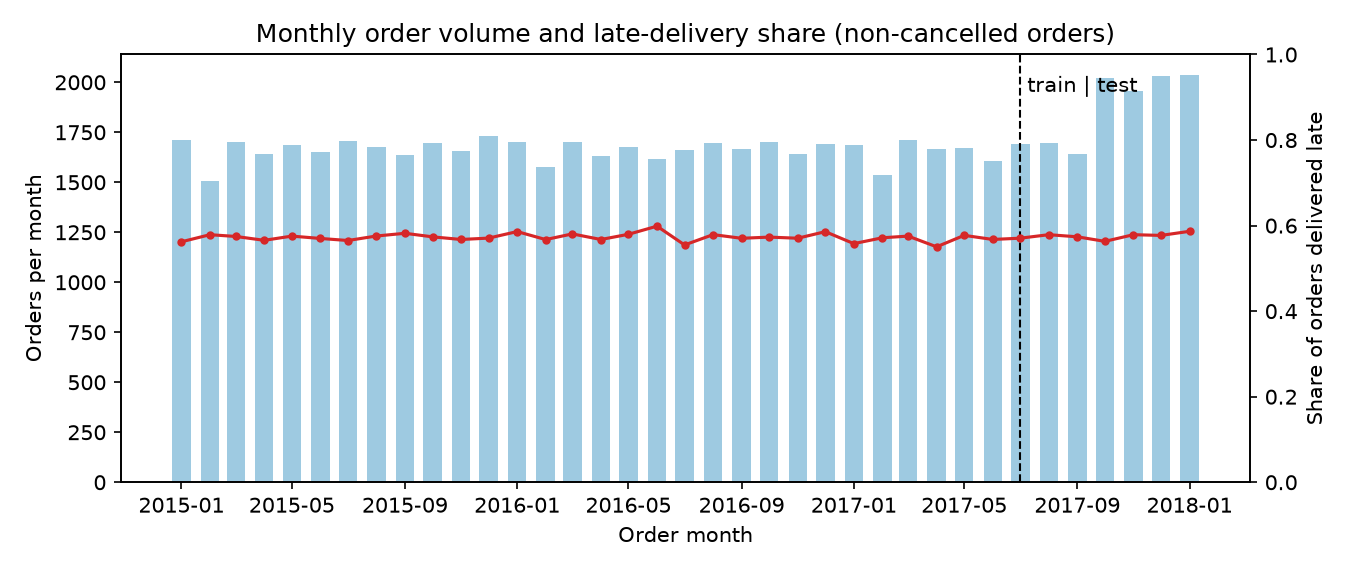
\includegraphics[width=0.85\linewidth]{01_monthly_volume_late_rate}
  \caption{Orders per month (bars, left axis) and share delivered late (line, right axis), non-cancelled orders. The dashed line marks the train/test split.}
  \label{fig:monthly}
\end{figure}

\begin{figure}[!htbp]
  \centering
  \begin{subfigure}[b]{0.47\linewidth}
    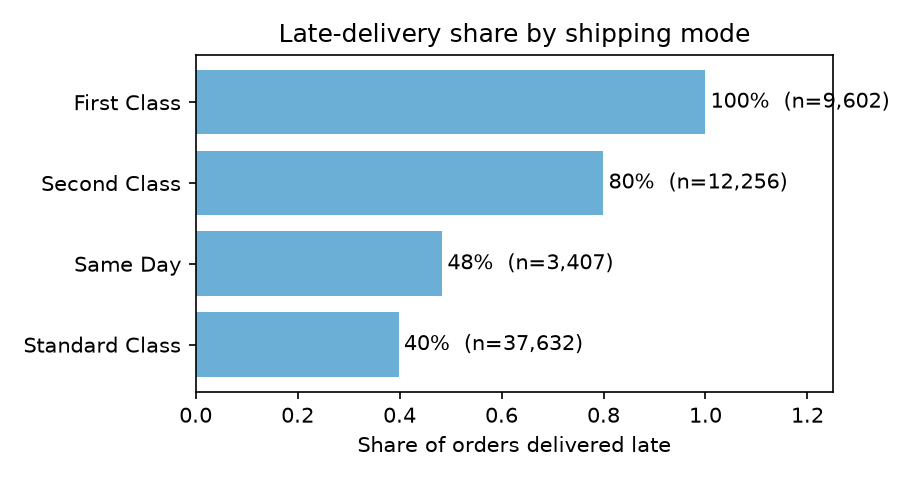
\includegraphics[width=\linewidth]{02_late_rate_by_mode}
    \caption{Late share by shipping mode (all periods).}
  \end{subfigure}\hfill
  \begin{subfigure}[b]{0.51\linewidth}
    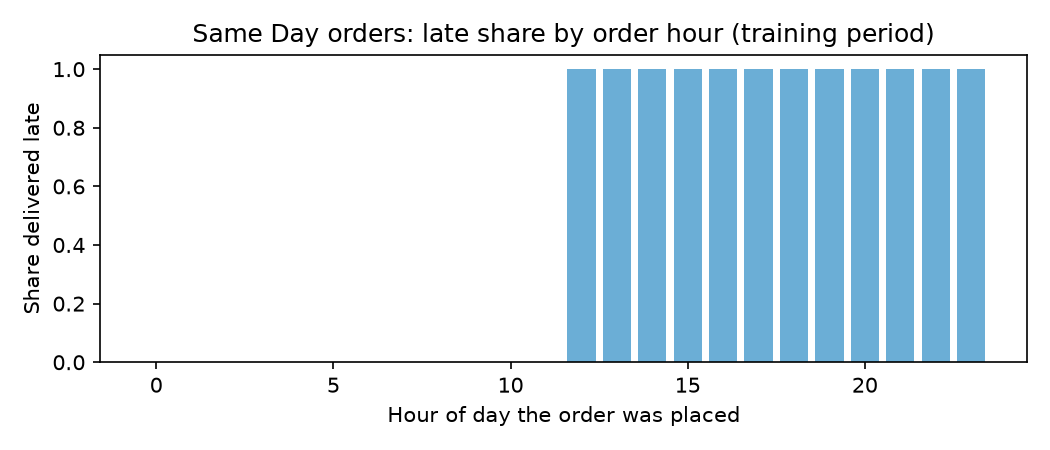
\includegraphics[width=\linewidth]{02b_same_day_late_by_hour}
    \caption{Same Day late share by order hour (training period).}
  \end{subfigure}
  \caption{The label is concentrated by shipping mode. Within Same Day it depends only on the hour of ordering.}
  \label{fig:mode}
\end{figure}

\subsection{Is the outcome operational? A realism check}
\label{subsec:realism}
Because the label is so concentrated, we tested whether transit time depends on anything real.
The results (\Cref{tab:realism}) show it does not. Transit days are a deterministic function of
fields with no operational meaning, and order timestamps are spaced in multiples of 21
minutes. The delivery timings in this dataset were almost certainly generated by an algorithm.
The dataset is on the approved list, so we keep it, but we treat this finding as a central
limitation (\Cref{sec:limitations}). It is also the reason we compare every model against the
lookup table rather than only against a weak rule.

\begin{table}[!htbp]
  \centering
  \caption{Realism checks on the 62{,}897 orders that were not cancelled.}
  \label{tab:realism}
  \footnotesize
  \begin{tabular}{l r}
    \toprule
    \textbf{Check} & \textbf{Share of orders matching} \\
    \midrule
    Standard and Second Class: real days $= (\text{Order Id} - 1) \bmod 5 + 2$ & 100.0\% \\
    First Class: real days $= 2$                                          & 100.0\% \\
    Same Day: late $\iff$ order placed at or after 12:00                   & 100.0\% \\
    Gap between consecutive orders is a multiple of 21 minutes             & 97.5\% \\
    \bottomrule
  \end{tabular}
\end{table}

\section{Data preparation}
\label{sec:prep}

\Cref{tab:prep} lists every preparation decision. All of them are implemented in
\tcode{src/data\_prep.py} and in the scikit-learn pipeline.

\begin{table}[!htbp]
  \centering
  \caption{Preparation decisions, their justification, and what each one risks.}
  \label{tab:prep}
  \footnotesize
  \begin{tabularx}{\linewidth}{>{\raggedright\arraybackslash}p{3.6cm} X}
    \toprule
    \textbf{Decision} & \textbf{Why, and what it risks} \\
    \midrule
    Drop 7{,}754 cancelled or suspected-fraud lines &
      These orders are never delivered, so there is no delivery decision for them. We assume
      the cancellation or fraud check happens before dispatch. \\
    Aggregate lines to orders &
      The decision is per order. Keeping lines would count multi-line orders several times and
      let lines of one order fall on both sides of a CV split. \\
    Order-level features &
      Lines, quantity, value, discount, maximum unit price, number of categories, profit,
      margin, and the department and category of the highest-value line. \\
    Calendar features &
      Weekday, hour and month of the order. The raw timestamp and \tcode{Order Id} are
      \emph{not} used, because they encode the order sequence, and the sequence determines the
      outcome here (\Cref{tab:realism}). \\
    History features &
      Prior order count and smoothed prior late rate, $(\text{late}+2.5)/(n+5)$, per customer,
      city, and city $\times$ mode. A past order counts only once its outcome was known. \\
    Drop PII and empty columns &
      Email, password, names, street and zip codes; \tcode{Product Description},
      \tcode{Order Zipcode} and \tcode{Product Image}. \\
    Keep outliers &
      They are genuine prices and losses, and trees are insensitive to them. \\
    Encoding and scaling &
      One-hot encoding for 6 low-cardinality categoricals (levels with fewer than 20 orders are
      pooled). Target encoding\cite{micci2001}, cross-fitted over 5 folds, for country (164),
      city (3{,}585) and category (50). Median imputation. Standard scaling for non-tree
      models only. \\
    \bottomrule
  \end{tabularx}
\end{table}

\paragraph{Leakage risks specific to this dataset and how each is avoided.}
\begin{enumerate}
  \item \textbf{\tcode{shipping date (DateOrders)}} looks like a dispatch date. In fact it equals the
        order date plus the \emph{real} transit days in 97.4\% of rows, so it encodes the outcome.
        It is excluded, together with \tcode{Days for shipping (real)}, \tcode{Delivery Status}
        and \tcode{Order Status}.
  \item \textbf{Order sequence.} Transit days follow \tcode{Order Id} modulo 5, so a model given
        the order ID or the raw timestamp could learn how the data was generated. Neither is a
        feature, and \tcode{run\_all.py} stops if one is ever added.
  \item \textbf{History features.} A naive ``past late rate'' would include orders that had not
        yet been delivered. We count a past order only after its order date + real transit
        days + 1 day.
  \item \textbf{Preprocessing.} Imputers, scalers and encoders sit inside the \tcode{Pipeline} and
        are refit on the training part of every fold. Target encoding is also cross-fitted
        within the training data.
\end{enumerate}

\section{Method}
\label{sec:method}

We compare six models from four families. Three of them (trees, SVM and neural networks) are
taught in Weeks 6--13. The four baselines from \Cref{sec:problem} are not counted as model
families. All models share the same features and the same preprocessing pipeline, built with
scikit-learn\cite{pedregosa2011}.
\Cref{app:parameters} gives the full settings.

\begin{table}[!htbp]
  \centering
  \caption{Models compared and the reason each was chosen.}
  \label{tab:models}
  \small
  \footnotesize
  \begin{tabularx}{\linewidth}{l l X}
    \toprule
    \textbf{Model} & \textbf{Family} & \textbf{Why it is here} \\
    \midrule
    Logistic regression      & linear          & Transparent reference; if it matches the others, the signal is simple. \\
    Decision tree (depth 6)  & trees (Wk 6)    & Rules a planner can check; depth from a sweep (\Cref{app:parameters}). \\
    Random forest (300 trees) & trees, bagging & Interactions such as city $\times$ mode, lower variance\cite{breiman2001}. \\
    Gradient boosting        & trees, boosting & Strongest tabular learner\cite{friedman2001}; finds any weak signal. \\
    SVM, RBF kernel          & SVM (Wk 8)      & Margin-based bias; 600-component Nystr\"om map\cite{williams2001} + linear SVM, since exact RBF is $O(n^2)$. \\
    MLP (64--32)             & ANN (Wk 7)      & Smooth non-linear effects; L2 penalty, early stopping. \\
    \bottomrule
  \end{tabularx}
\end{table}

\subsection{From scores to decisions}
\label{subsec:policy}
A score by itself is not a decision, so every method is turned into a flagging
\emph{policy}:
\begin{itemize}
  \item \textbf{Probabilistic methods} (lookup table, logistic regression, trees, MLP) use the
        expected-value rule\cite{elkan2001}: flag an order when the late-delivery cost it is
        expected to avoid exceeds the action cost,
        \begin{equation}
          \hat p \cdot \underbrace{0.5}_{\text{avoided}} \cdot \underbrace{0.10\,v}_{\text{miss cost}} > \underbrace{\usd{10}}_{\text{action}}
          \quad\Longleftrightarrow\quad \hat p \cdot v > \usd{200}.
          \label{eq:ev}
        \end{equation}
        No threshold is tuned, but the rule needs calibrated probabilities, so we report the
        Brier score.
  \item \textbf{SVM} scores are not probabilities. Its threshold is the one that maximises
        saving on out-of-fold training scores.
  \item \textbf{Rules} flag exactly the orders they select. The majority baseline flags every
        order.
\end{itemize}
The cost model then turns each policy into dollars per week (\Cref{tab:costs}).

\section{Validation design}
\label{sec:validation}

\paragraph{Split.} The data is split \textbf{by time and never shuffled}. Orders placed before
2017-07-01 form the training set (49{,}826 orders, 57.2\% late). Orders from 2017-07-01 to
2018-01-31 form the test set (13{,}071 orders, 57.6\% late, 30.6 weeks). Nothing chosen during
development used the test set. That includes model settings, the SVM threshold, the Same Day
cut-off hour and the choice of best model. The test set was scored once, at the end.

\paragraph{Cross-validation.} We use rolling-origin validation\cite{bergmeir2012} with
\tcode{TimeSeriesSplit(5)} on the training period. Each fold trains on all earlier orders and
validates on the next block of about 8{,}300 orders. Every table reports the mean and standard
deviation across the 5 folds. On the test set, 95\% intervals come from 200 bootstrap resamples,
and all methods share the same resamples.

\paragraph{Metrics and why.}
\begin{itemize}
  \item \textbf{PR-AUC (average precision)}, the headline metric: how pure the flagged list is at
        every alert rate\cite{saito2015}. scikit-learn scores a block of tied scores at its pooled
        precision, which penalises few-valued methods (lookup table: 0.805 instead of 0.859 on
        test), so we break ties at random (mean of 5 draws). Continuous scores are unaffected.
  \item \textbf{ROC-AUC}, also computed within each shipping mode, to isolate any signal beyond
        what the rules capture. \textbf{Recall and precision at a 35\% alert rate}, roughly the
        capacity implied by Rule A.
  \item \textbf{Net saving per order and per week} under \Cref{tab:costs}, the metric tied to the
        decision. The \textbf{Brier score} checks calibration for the expected-value policy.
\end{itemize}
Accuracy is reported only alongside these metrics.

\section{Results}
\label{sec:results}

\subsection{Cross-validation on the training period}
\begin{table}[!htbp]
  \centering
  \caption{Rolling-origin CV, 5 folds: mean $\pm$ standard deviation across folds. PR-AUC is computed with ties broken at random. Recall and precision are measured at a 35\% alert rate. Best value in bold.}
  \label{tab:cv}
  \footnotesize
  \setlength{\tabcolsep}{3pt}
  \begin{tabular}{l c c c c c}
    \toprule
    \textbf{Method} & \textbf{PR-AUC} & \textbf{ROC-AUC} & \textbf{Recall@35\%} & \textbf{Prec.@35\%} & \textbf{Brier} \\
    \midrule
    Majority class           & $0.573 \pm 0.003$ & $0.500 \pm 0.000$ & $0.348 \pm 0.007$ & $0.569 \pm 0.010$ & $0.245$ \\
    Rule A: First/Second     & $0.790 \pm 0.004$ & $0.724 \pm 0.003$ & $0.540 \pm 0.002$ & $0.884 \pm 0.005$ & -- \\
    Rule B: + Same Day cut-off & $0.806 \pm 0.003$ & $0.745 \pm 0.002$ & $0.546 \pm 0.003$ & $0.894 \pm 0.004$ & -- \\
    Lookup table             & $\mathbf{0.855 \pm 0.002}$ & $\mathbf{0.774 \pm 0.002}$ & $0.550 \pm 0.002$ & $0.901 \pm 0.004$ & $\mathbf{0.175}$ \\
    \midrule
    Logistic regression      & $0.837 \pm 0.002$ & $0.743 \pm 0.003$ & $0.542 \pm 0.001$ & $0.886 \pm 0.004$ & $0.190$ \\
    Decision tree            & $0.854 \pm 0.005$ & $0.770 \pm 0.006$ & $0.550 \pm 0.002$ & $0.901 \pm 0.003$ & $0.180$ \\
    Random forest            & $0.850 \pm 0.003$ & $0.769 \pm 0.004$ & $0.549 \pm 0.003$ & $0.899 \pm 0.002$ & $0.179$ \\
    Gradient boosting        & $0.853 \pm 0.003$ & $0.771 \pm 0.004$ & $\mathbf{0.551 \pm 0.003}$ & $\mathbf{0.901 \pm 0.002}$ & $0.179$ \\
    SVM (RBF, Nystr\"om)     & $0.840 \pm 0.005$ & $0.753 \pm 0.010$ & $0.546 \pm 0.003$ & $0.893 \pm 0.005$ & -- \\
    MLP                      & $0.845 \pm 0.007$ & $0.761 \pm 0.011$ & $0.544 \pm 0.006$ & $0.891 \pm 0.008$ & $0.186$ \\
    \bottomrule
  \end{tabular}
\end{table}

All six models beat the majority class and both rules; none beats the lookup table. The gaps
between the table, the decision tree and gradient boosting (0.001--0.002) are below one fold
SD, so they are tied. The decision tree is formally the best model by mean CV PR-AUC and is
carried forward. Folds are very stable (\Cref{fig:cvbox} in \Cref{app:figures}), which is expected when the label depends on only two
fields.


\subsection{Held-out test period (2017-07 to 2018-01)}
\begin{table}[!htbp]
  \centering
  \caption{Test-set results, with 95\% bootstrap intervals (200 resamples) in brackets. Policies are defined in \Cref{subsec:policy}. Saving is measured against taking no action, in USD per order.}
  \label{tab:test}
  \footnotesize
  \setlength{\tabcolsep}{2.5pt}
  \begin{tabular}{l c c c c c}
    \toprule
    \textbf{Method} & \textbf{PR-AUC} & \textbf{ROC-AUC} & \textbf{Alert rate} & \textbf{Recall / Prec.} & \textbf{Saving/order} \\
    \midrule
    Majority (flag all)  & 0.577 [0.567, 0.585] & 0.500 & 100\% & 1.00 / 0.58 & 2.31 [1.94, 2.57] \\
    Rule A               & 0.794 [0.784, 0.802] & 0.724 & 35\%  & 0.54 / 0.89 & 3.23 [3.01, 3.41] \\
    Rule B               & 0.813 [0.803, 0.821] & 0.750 & 38\%  & 0.59 / 0.90 & 3.51 [3.27, 3.69] \\
    Lookup table         & 0.859 [0.853, 0.864] & 0.777 & 44\%  & 0.53 / 0.69 & 5.61 [5.30, 5.86] \\
    \midrule
    Logistic regression  & 0.845 [0.838, 0.852] & 0.757 & 44\%  & 0.51 / 0.67 & 5.48 [5.18, 5.73] \\
    Decision tree        & 0.861 [0.855, 0.867] & 0.780 & 44\%  & 0.53 / 0.69 & 5.60 [5.29, 5.84] \\
    Random forest        & 0.858 [0.851, 0.864] & 0.782 & 45\%  & 0.53 / 0.68 & 5.58 [5.28, 5.84] \\
    Gradient boosting    & 0.860 [0.854, 0.867] & 0.781 & 44\%  & 0.53 / 0.69 & 5.62 [5.32, 5.87] \\
    SVM (RBF, Nystr\"om) & 0.850 [0.842, 0.856] & 0.770 & 99\%  & 1.00 / 0.58 & 2.39 [2.04, 2.65] \\
    MLP                  & 0.858 [0.851, 0.864] & 0.778 & 42\%  & 0.51 / 0.69 & 5.56 [5.25, 5.81] \\
    \bottomrule
  \end{tabular}
\end{table}

The test results repeat the CV ranking, with overlapping intervals among the lookup table and
the tree models. The expected-value policies save about \usd{5.6} per order, against \usd{3.5}
for the best rule. They flag \emph{fewer} late orders than the rules (recall 0.53 against 0.59)
but choose them by value: a cheap First Class order is not worth a \usd{10} action. The SVM
threshold chosen on training folds flags almost everything, and so it gives up most of the
saving. This is a known weakness of models without calibrated probabilities. \Cref{fig:pr} in \Cref{app:figures} shows the precision--recall curves.


\subsection{Is there any signal beyond shipping mode?}
\Cref{tab:within} answers the key question. Inside Second Class and Standard Class, which
together hold 79\% of test orders, every model ranks orders at chance level. The only
within-mode signal is Same Day, and the models find it only because they rediscover the noon
cut-off. First Class has no variation to explain.

\begin{table}[!htbp]
  \centering
  \caption{Test ROC-AUC computed within each shipping mode (0.5 = chance). First Class is always late, so its AUC is undefined.}
  \label{tab:within}
  \small
  \begin{tabular}{l r r c c c c}
    \toprule
    \textbf{Mode} & \textbf{Orders} & \textbf{Late} & \textbf{LogReg} & \textbf{Tree} & \textbf{Gr.\ boost.} & \textbf{MLP} \\
    \midrule
    Same Day       &   731 & 54\%  & 0.903 & 1.000 & 1.000 & 0.999 \\
    Second Class   & 2{,}586 & 81\% & 0.499 & 0.478 & 0.471 & 0.501 \\
    Standard Class & 7{,}780 & 39\% & 0.519 & 0.511 & 0.513 & 0.509 \\
    First Class    & 1{,}974 & 100\% & -- & -- & -- & -- \\
    \bottomrule
  \end{tabular}
\end{table}

\paragraph{Drift check.} When the test period is split at 2017-10-01 (\Cref{tab:drift}), PR-AUC
holds for every method, but the saving per order falls from \usd{9.8} to \usd{3.0} as the median
order value falls from \usd{610} to \usd{253}. The ranking is stable; the dollar value is not.

\section{Interpretation}
\label{sec:interpretation}

\paragraph{What drives the model.} We measured permutation importance on the test set as the
drop in PR-AUC when one feature is shuffled (\Cref{fig:perm}). For the decision tree, three
features carry almost everything: shipping mode (0.164), scheduled days (0.087, which is the
same information as mode) and order hour (0.053). Every other feature scores below 0.001. For
gradient boosting the picture is the same: mode 0.283, hour 0.035, and nothing else above 0.002.
Destination, customer history, order value, discount and product category do not matter.

\begin{figure}[!htbp]
  \centering
  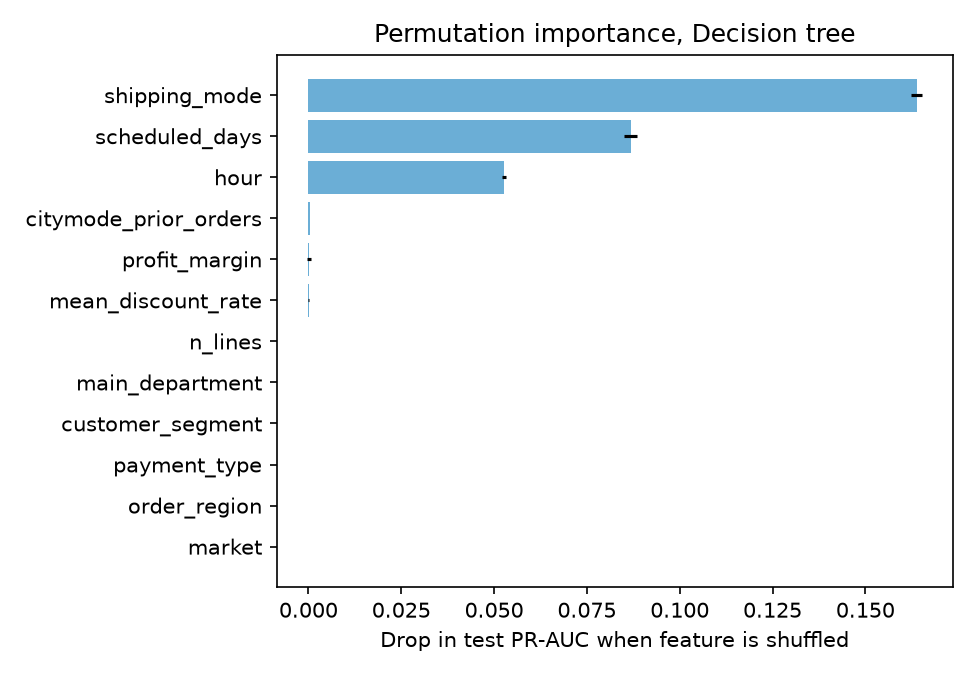
\includegraphics[width=0.5\linewidth]{06_permutation_importance}
  \caption{Permutation importance for the decision tree: mean drop in test PR-AUC over 5 shuffles, with error bars showing one standard deviation.}
  \label{fig:perm}
\end{figure}

\paragraph{Tree structure.} The depth-3 tree in \Cref{fig:tree} reads as a policy manual. The
first split separates Standard Class (40\% late) from the rest. On the left, the tree
isolates Same Day (\tcode{scheduled\_days} $\le 0.5$) and splits it at \tcode{hour} $\le 11.5$
into leaves that are 0\% and 100\% late. First Class becomes a 100\%-late leaf, and Second Class
a leaf that is 80\% late. On the right, the splits on target-encoded city and city $\times$ mode
history move the late share only between 39\% and 43\%. That is noise, and these leaves
disappear from the importance ranking.

\begin{figure}[!htbp]
  \centering
  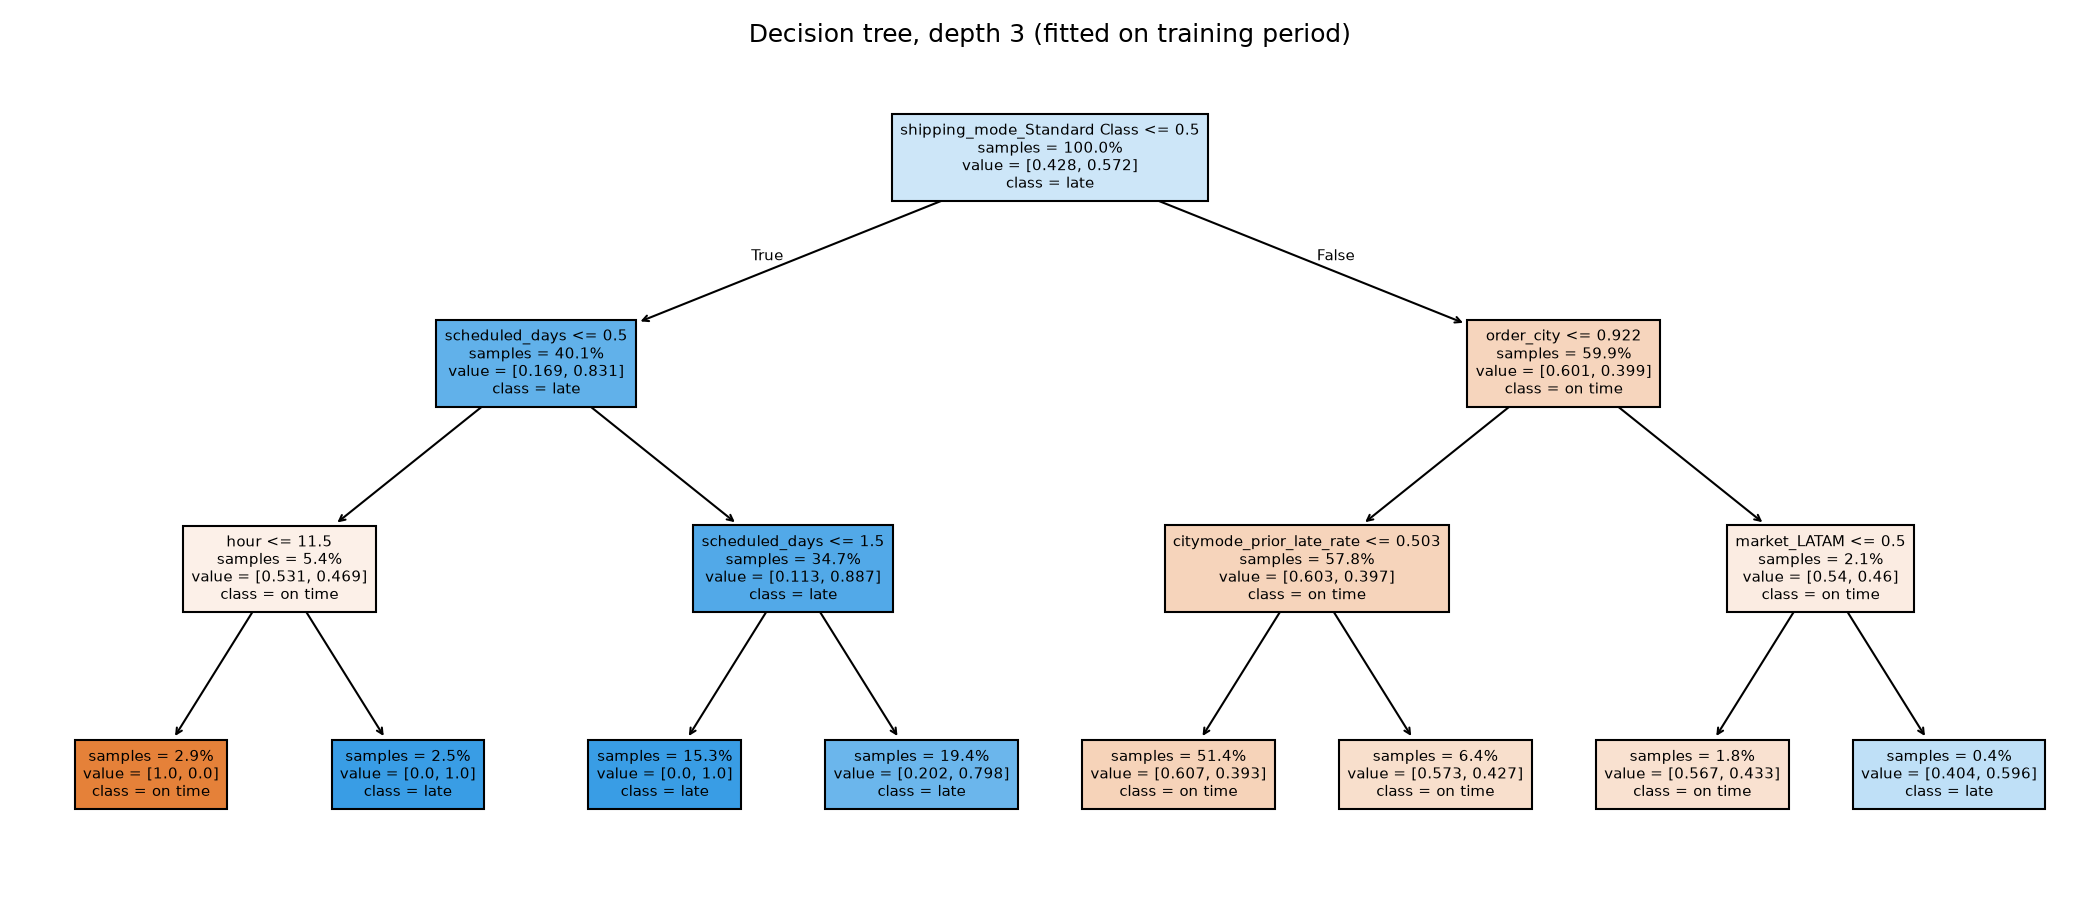
\includegraphics[width=0.85\linewidth]{07_decision_tree_depth3}
  \caption{Decision tree limited to depth 3, fitted on the training period. \tcode{value} gives the shares [on time, late]; \tcode{samples} is the share of training orders reaching each node.}
  \label{fig:tree}
\end{figure}

\paragraph{Does this make supply-chain sense?} Mostly, yes, and it points at the promise rather
than the order.
\begin{itemize}
  \item \textbf{First Class} is promised 1 day and always takes 2: a service-level design error,
        not a risk to predict.
  \item \textbf{Second Class and Standard} both take 2--6 days uniformly, mean 4.0
        (\Cref{tab:requote}). Second Class is \emph{not faster}, only promised as faster, and
        its buyers are late 80\% of the time.
  \item \textbf{Same Day} behaves like a warehouse with a 12:00 cut-off, which real fulfilment
        centres use; the fix is to show the cut-off at checkout.
  \item The \textbf{absence} of destination, customer or product effects is not plausible for
        real logistics. It is consistent with the realism checks (\Cref{subsec:realism}), so we
        read it as a property of the data.
\end{itemize}
The partial-dependence plots in \Cref{app:figures} confirm this. The average predicted late
probability jumps by about 6 points at 12:00. For order value, discount and city $\times$ mode
history it moves by at most 2 points, and a feature whose permutation importance is
essentially zero cannot turn that movement into better rankings.

\section{Recommendation}
\label{sec:recommendation}

\subsection{Action 1: fix the promises (largest effect)}
The cheapest intervention is to change the promise. \Cref{tab:scenarios} applies cumulative
changes to the test-period orders, using the noon cut-off learned on the training period.

\begin{table}[!htbp]
  \centering
  \caption{Promise scenarios on the test period (428 orders per week). Late cost is $0.10\times$ order value per late order.}
  \label{tab:scenarios}
  \footnotesize
  \setlength{\tabcolsep}{4pt}
  \begin{tabular}{l c c c c}
    \toprule
    \textbf{Scenario} & \textbf{Late share} & \textbf{Late/wk} & \textbf{Mean promise} & \textbf{Late cost/wk} \\
    \midrule
    Current (0/1/2/4 days)                          & 57.6\% & 246 & 2.93 d & \usd{10{,}520} \\
    A: Same Day after 12:00 promised next day       & 54.5\% & 233 & 2.96 d & \usd{10{,}020} \\
    B: A + First Class promised 2 days              & 39.4\% & 169 & 3.11 d & \usd{7{,}240} \\
    C: B + Second Class promised 4 days             & 31.5\% & 135 & 3.50 d & \usd{5{,}770} \\
    D: C + Second/Standard promised 6 days          & 0.0\%  & 0   & 5.09 d & \usd{0} \\
    \bottomrule
  \end{tabular}
\end{table}

\textbf{Recommended: scenario B, now.} First Class already takes exactly 2 days, so the new
promise costs no speed, and a checkout cut-off for Same Day is standard practice. B removes 77
late orders and about \usd{3{,}300} of late cost per week. Scenario C is a commercial decision:
Second Class is no faster than Standard, so DataCo should fix it or stop selling it as faster.
We do not recommend D, whose lost conversions the data cannot measure.

\subsection{Action 2: flag orders at release with the lookup table}
Some late orders remain after the promise change, so the planner still needs a daily list.
\Cref{fig:saving} plots weekly net saving against the share of orders flagged, with orders
ranked by $\hat p\times v$. The saving peaks at about a 45\% alert rate for both the lookup
table and the decision tree (\usd{2{,}400} per week). Beyond that point, each extra check costs
more than the late delivery it prevents. Rule B peaks earlier, at 25\% (\usd{1{,}810} per week),
because it cannot tell a Second Class order (80\% late) from a First Class one (100\% late).

\begin{figure}[!htbp]
  \centering
  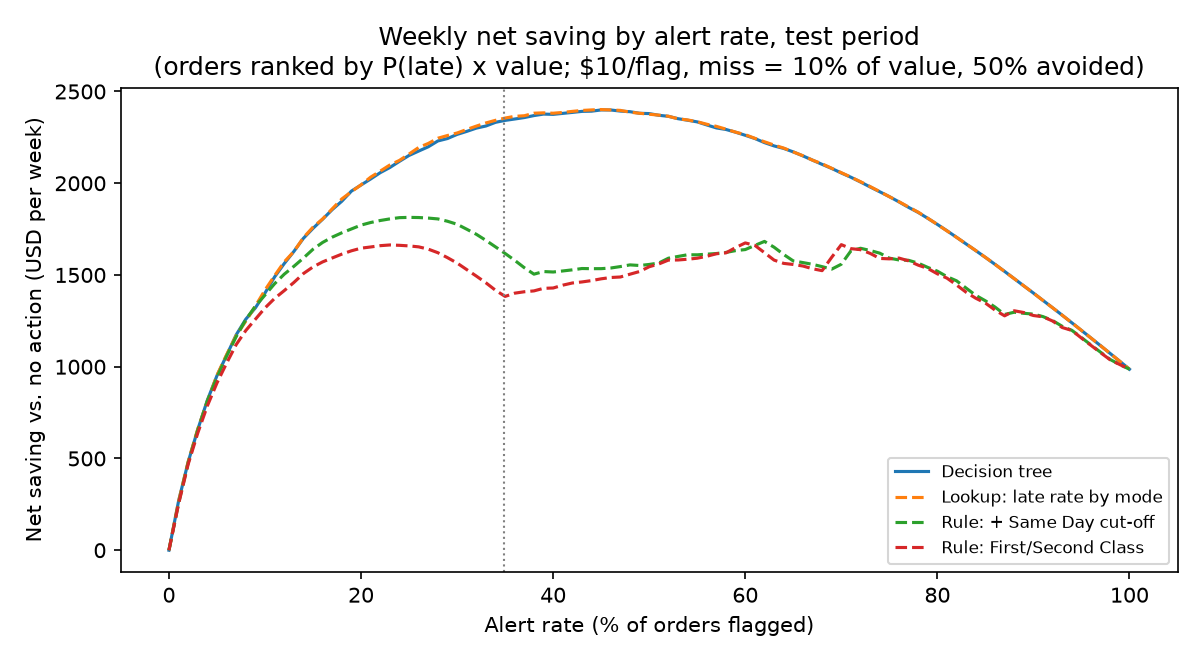
\includegraphics[width=0.66\linewidth]{05_saving_vs_alert_rate}
  \caption{Weekly net saving compared with taking no action, by alert rate, on the test period. The dotted line marks Rule A's alert rate.}
  \label{fig:saving}
\end{figure}

\begin{table}[!htbp]
  \centering
  \caption{Weekly operational effect of each policy on the test period (428 orders per week).}
  \label{tab:rec}
  \footnotesize
  \setlength{\tabcolsep}{3pt}
  \begin{tabular}{l c c c c c}
    \toprule
    \textbf{Policy} & \textbf{Flagged} & \textbf{Late caught} & \textbf{Late missed} & \textbf{False alarms} & \textbf{Net saving} \\
    \midrule
    Lookup table, EV rule & 187 & 129 & 117 & 57  & \usd{2{,}399} \\
    Decision tree, EV rule & 188 & 129 & 117 & 59  & \usd{2{,}393} \\
    Rule B (+ Same Day cut-off)        & 162 & 146 & 101 & 16  & \usd{1{,}503} \\
    Rule A (First/Second)              & 149 & 133 & 113 & 16  & \usd{1{,}381} \\
    Flag every order                   & 428 & 246 & 0   & 181 & \usd{986} \\
    \bottomrule
  \end{tabular}
\end{table}

\textbf{Recommended policy:} each morning, flag the orders for which
$P(\text{late})\times\text{order value} > \usd{200}$, where $P(\text{late})$ comes from the
five-row lookup table below. The expected workload is about \textbf{190 orders per week},
roughly 27 per day. That is about 16 hours of customer-service time per week, assuming 5
minutes per order. It catches 129 late orders per week and saves about \usd{900} per week more
than Rule B.

\begin{center}
  \small
  \begin{tabular}{l c c}
    \toprule
    \textbf{Cell (from training data)} & \textbf{$P(\text{late})$} & \textbf{Flag if order value exceeds} \\
    \midrule
    First Class; Same Day after 12:00 & 1.00 & \usd{200} \\
    Second Class                      & 0.80 & \usd{250} \\
    Standard Class                    & 0.40 & \usd{500} \\
    Same Day before 12:00             & 0.00 & never \\
    \bottomrule
  \end{tabular}
\end{center}

\textbf{Why the lookup table and not the model.} The tree and gradient boosting give the same
answer at extra cost: retraining, monitoring, and logic planners cannot check by eye. Across all
36 cost settings (action \usd{2}--\usd{20}, miss 5--20\% of value, 30--70\% avoided), the best model
and the table differ by $-\usd{24}$ to $+\usd{5}$ per week, while the table beats Rule B by
\usd{300}--\usd{5{,}500} per week. At a \usd{2} action cost the optimal alert rate rises to 60--90\%.

\paragraph{Size of the effect.} Under the stated assumptions, scenario B avoids about
\textbf{\usd{3{,}300} per week} of late-delivery cost, and the flagging policy saves a further
\textbf{\usd{900} per week} over the current-practice proxy: roughly \usd{200}k per year at 2017
volumes. Because the saving scales with order value, which fell by two-thirds in late 2017, we
would quote it as ``tens to low hundreds of thousands of dollars per year''.

\section{Limitations}
\label{sec:limitations}

\paragraph{What the model cannot do.} It cannot say \emph{which} Standard or Second Class orders
(79\% of volume) will be late; within those modes it is no better than a coin. It does not
predict the \emph{size} of a delay.

\paragraph{Where the data is unrepresentative.}
\begin{itemize}
  \item \textbf{Synthetic outcome.} Transit days follow the order ID modulo 5 (\Cref{tab:realism}).
        ``Only mode and hour matter'' may describe the data generator, not DataCo's network; on
        real data, destination, carrier and warehouse load would very likely carry signal. The
        pipeline is ready for such data, but the ``use the lookup table'' conclusion may not
        transfer.
  \item \textbf{Drift after 2017-Q4.} Ranking quality held, but the saving per order fell from
        \usd{9.8} to \usd{3.0}.
  \item \textbf{Costs are assumed.} The \emph{choice} of policy is robust across the sensitivity
        grid; the size of the saving is not.
  \item \textbf{Promise changes affect demand.} Longer promises may reduce conversion, which the
        data cannot measure. Scenario B only aligns promises with what already happens;
        C and D need a controlled test.
\end{itemize}

\paragraph{What must be true for the recommendation to hold.} Real transit times depend mainly
on mode and cut-off; customers accept a 2-day First Class promise; a flagged order avoids about
half of the late-delivery cost.

\paragraph{With more time or data.} We would refit the pipeline on carrier and warehouse records
(dispatch times, carrier, distance), A/B-test the promise change in one market, estimate the
effect of an action from past interventions instead of assuming 50\%, and add a regression
model for the size of the delay.

\section{Contribution table}
\label{sec:contribution}

\begin{table}[!htbp]
  \centering
  \caption{Lead responsibilities.}
  \label{tab:contribution}
  \footnotesize
  \begin{tabularx}{\linewidth}{l l X}
    \toprule
    \textbf{Member} & \textbf{ID} & \textbf{Led} \\
    \midrule
    Lê Thanh Duy           & 2352178 & Problem framing, cost model, recommendation (\Cref{sec:problem,sec:recommendation}) \\
    Lương Trương Quang Huy & 2352385 & Data audit, quality and realism checks (\Cref{sec:data}) \\
    Lê Tuấn Tài            & 2312997 & Order-level features, leakage control, history features (\Cref{sec:prep}) \\
    Nguyễn Quốc Đăng Khoa  & 2311625 & Validation design, time split, bootstrap intervals (\Cref{sec:validation}) \\
    Nguyễn Lê Chí Kiên     & 2352643 & Tree models and interpretation (\Cref{sec:method,sec:interpretation}) \\
    Phạm Hải Nam           & 2352783 & SVM and MLP models, results tables, presentation (\Cref{sec:results}) \\
    \bottomrule
  \end{tabularx}
\end{table}


\renewcommand{\bibfont}{\footnotesize}
\setlength{\bibsep}{0pt plus 1pt}
\bibliographystyle{plainnat}
\bibliography{refs/refs}

\clearpage
\appendix
\section{Data dictionary}
\label{app:dictionary}

All 28 features used, plus the target, at order level (62{,}897 orders). No feature has missing
values after preparation. The raw source columns are described in the column description file shipped with the dataset.

\begin{footnotesize}
\begin{longtable}{>{\raggedright\arraybackslash}p{4.6cm} >{\raggedright\arraybackslash}p{2.6cm} >{\raggedright\arraybackslash}p{5.2cm} r}
  \caption{Data dictionary of the order-level table.}\label{tab:dictionary}\\
  \toprule
  \textbf{Feature} & \textbf{Type} & \textbf{Description} & \textbf{Unique} \\
  \midrule
  \endfirsthead
  \toprule
  \textbf{Feature} & \textbf{Type} & \textbf{Description} & \textbf{Unique} \\
  \midrule
  \endhead
    \tcode{shipping\_mode} & categorical & Shipping mode chosen at order (Standard/Second/First/Same Day) & 4 \\
    \tcode{market} & categorical & Destination market (5 values) & 5 \\
    \tcode{order\_region} & categorical & Destination region (23 values) & 23 \\
    \tcode{customer\_segment} & categorical & Consumer / Corporate / Home Office & 3 \\
    \tcode{payment\_type} & categorical & Transaction type: DEBIT{,} TRANSFER{,} PAYMENT{,} CASH & 4 \\
    \tcode{main\_department} & categorical & Department of the order's highest-value line & 11 \\
    \tcode{order\_country} & categorical{,} target-encoded & Destination country & 164 \\
    \tcode{order\_city} & categorical{,} target-encoded & Destination city & 3{,}585 \\
    \tcode{main\_category} & categorical{,} target-encoded & Product category of the highest-value line & 50 \\
    \tcode{scheduled\_days} & numeric & Promised shipping days (fixed by mode: 0/1/2/4) & 4 \\
    \tcode{n\_lines} & numeric & Number of order lines & 5 \\
    \tcode{total\_qty} & numeric & Total units ordered & 24 \\
    \tcode{order\_value} & numeric{,} USD & Sum of line Sales (before discount) & 18{,}647 \\
    \tcode{total\_discount} & numeric{,} USD & Sum of line discounts & 20{,}182 \\
    \tcode{mean\_discount\_rate} & numeric & Mean line discount rate & 4{,}513 \\
    \tcode{max\_unit\_price} & numeric{,} USD & Highest unit price in the order & 75 \\
    \tcode{n\_categories} & numeric & Distinct product categories in the order & 5 \\
    \tcode{order\_profit} & numeric{,} USD & Sum of 'Benefit per order' over lines & 52{,}398 \\
    \tcode{profit\_margin} & numeric & order\_profit / order\_value & 58{,}088 \\
    \tcode{weekday} & numeric & Day of week of order (0 = Monday) & 7 \\
    \tcode{hour} & numeric & Hour of day of order & 24 \\
    \tcode{month} & numeric & Month of order & 12 \\
    \tcode{cust\_prior\_orders} & numeric & Customer's earlier orders whose outcome was already known & 15 \\
    \tcode{cust\_prior\_late\_rate} & numeric & Smoothed late share of those orders & 72 \\
    \tcode{city\_prior\_orders} & numeric & Earlier orders to the same city with known outcome & 633 \\
    \tcode{city\_prior\_late\_rate} & numeric & Smoothed late share of those orders & 3{,}653 \\
    \tcode{citymode\_prior\_orders} & numeric & Same{,} for city x shipping mode & 399 \\
    \tcode{citymode\_prior\_late\_rate} & numeric & Smoothed late share of those orders & 2{,}485 \\
    \tcode{late} & binary target & Late\_delivery\_risk: 1 if real shipping days > scheduled days & 2 \\
  \bottomrule
\end{longtable}
\end{footnotesize}

\section{Model settings and tuning}
\label{app:parameters}

\begin{table}[H]
  \centering
  \caption{Full parameter settings (scikit-learn 1.9.1, \tcode{random\_state=42}). Unlisted parameters are library defaults.}
  \label{tab:params}
  \footnotesize
  \begin{tabularx}{\linewidth}{l X}
    \toprule
    \textbf{Model} & \textbf{Settings} \\
    \midrule
    Majority class      & \tcode{DummyClassifier(strategy="prior")} \\
    Rule A / Rule B     & Custom estimator. Rule B learns its cut-off in \tcode{fit()} as the first hour whose Same Day late share exceeds 50\% (12:00 on the training set). \\
    Lookup table        & Custom estimator: mean late share per cell (4 modes, with Same Day split at the learned cut-off). \\
    Logistic regression & \tcode{C=1.0, max\_iter=2000}; scaled inputs \\
    Decision tree       & \tcode{max\_depth=6, min\_samples\_leaf=50}; unscaled inputs \\
    Random forest       & \tcode{n\_estimators=300, min\_samples\_leaf=20, max\_features="sqrt"} \\
    Gradient boosting   & \tcode{HistGradientBoostingClassifier(learning\_rate=0.05, max\_iter=300, max\_leaf\_nodes=31, early\_stopping=True)} \\
    SVM                 & \tcode{Nystroem(kernel="rbf", gamma=0.02, n\_components=600)} $\rightarrow$ \tcode{LinearSVC(C=0.1)}; scaled inputs \\
    MLP                 & \tcode{hidden\_layer\_sizes=(64, 32), alpha=1e-3, learning\_rate\_init=1e-3, max\_iter=200, early\_stopping=True}; scaled inputs \\
    Preprocessing       & \tcode{OneHotEncoder(min\_frequency=20,} \tcode{handle\_unknown="infrequent\_if\_exist")}; \tcode{TargetEncoder(target\_type="binary", cv=KFold(5, shuffle=True))}; \tcode{SimpleImputer(median)}; \tcode{StandardScaler} (non-tree models only) \\
    \bottomrule
  \end{tabularx}
\end{table}

\begin{table}[H]
  \centering
  \caption{Decision-tree depth sweep (rolling-origin CV, 5 folds, standard average precision). Most of the gain with depth comes from deeper trees splitting tied leaves into many small ones, which standard AP rewards (\Cref{sec:validation}); with ties broken, depth 6 already scores 0.854. We kept depth 6 for readability.}
  \label{tab:depth}
  \small
  \begin{tabular}{l c c c c c c c}
    \toprule
    \tcode{max\_depth} & 2 & 3 & 4 & 6 & 8 & 12 & none \\
    \midrule
    PR-AUC mean & 0.760 & 0.808 & 0.818 & 0.832 & 0.839 & 0.846 & 0.847 \\
    PR-AUC SD   & 0.008 & 0.005 & 0.010 & 0.009 & 0.006 & 0.003 & 0.002 \\
    \bottomrule
  \end{tabular}
\end{table}

\section{Additional results}
\label{app:figures}

\begin{table}[H]
  \centering
  \caption{Actual transit days by mode in the training period, and the late share that would result if $p$ days were promised. Current promises are shown in bold.}
  \label{tab:requote}
  \small
  \setlength{\tabcolsep}{4pt}
  \begin{tabular}{l r c c c c c c c c}
    \toprule
    & & \multicolumn{2}{c}{\textbf{Real days}} & \multicolumn{6}{c}{\textbf{Late share if promise = $p$ days}} \\
    \cmidrule(lr){3-4}\cmidrule(lr){5-10}
    \textbf{Mode} & \textbf{Orders} & mean & range & $p=0$ & 1 & 2 & 3 & 4 & 6 \\
    \midrule
    Same Day       & 2{,}676  & 0.47 & 0--1 & \textbf{0.47} & 0.00 & 0 & 0 & 0 & 0 \\
    First Class    & 7{,}628  & 2.00 & 2--2 & 1.00 & \textbf{1.00} & 0.00 & 0 & 0 & 0 \\
    Second Class   & 9{,}670  & 4.00 & 2--6 & 1.00 & 1.00 & \textbf{0.80} & 0.60 & 0.40 & 0.00 \\
    Standard Class & 29{,}852 & 4.00 & 2--6 & 1.00 & 1.00 & 0.80 & 0.60 & \textbf{0.40} & 0.00 \\
    \bottomrule
  \end{tabular}
\end{table}

\begin{figure}[H]
  \centering
  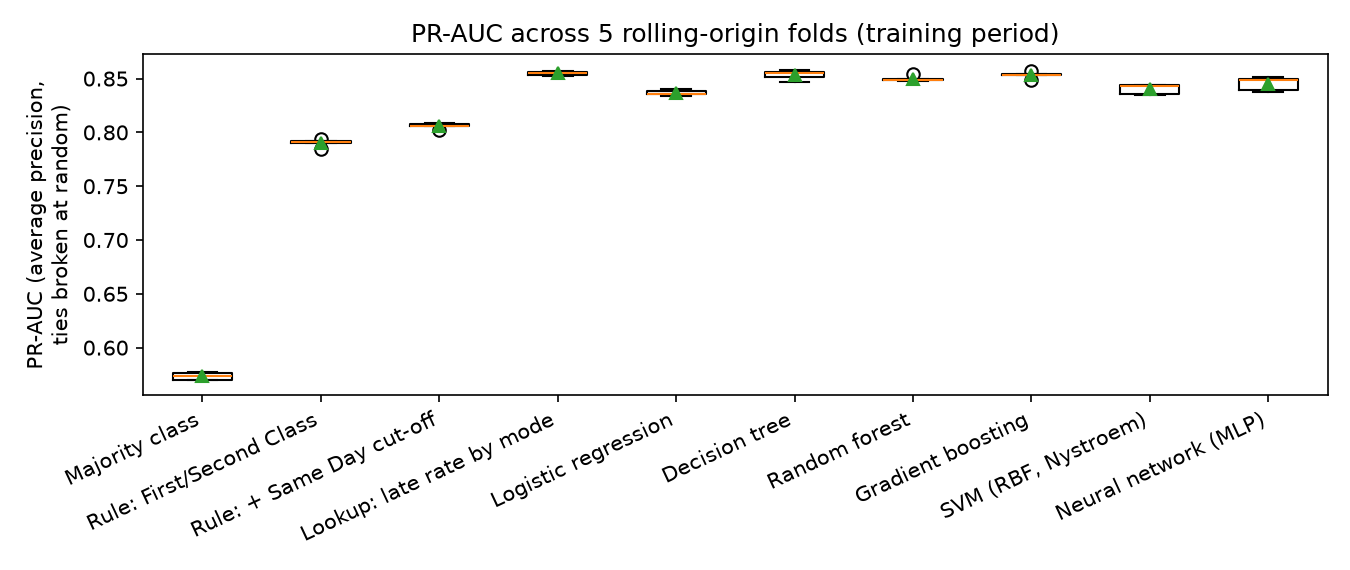
\includegraphics[width=0.85\linewidth]{03_cv_pr_auc_boxplot}
  \caption{PR-AUC (ties broken at random) across the 5 rolling-origin folds; triangles mark the mean.}
  \label{fig:cvbox}
\end{figure}

\begin{figure}[H]
  \centering
  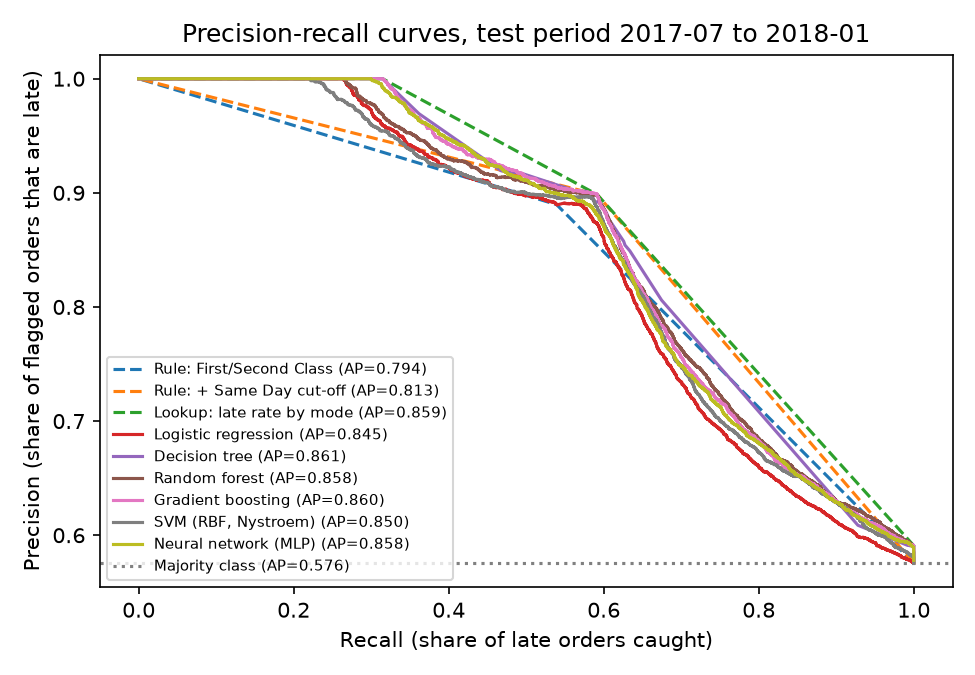
\includegraphics[width=0.62\linewidth]{04_test_pr_curves}
  \caption{Precision--recall curves on the test period. Dashed lines are baselines; the AP values in the legend are computed with ties broken at random.}
  \label{fig:pr}
\end{figure}

\begin{figure}[H]
  \centering
  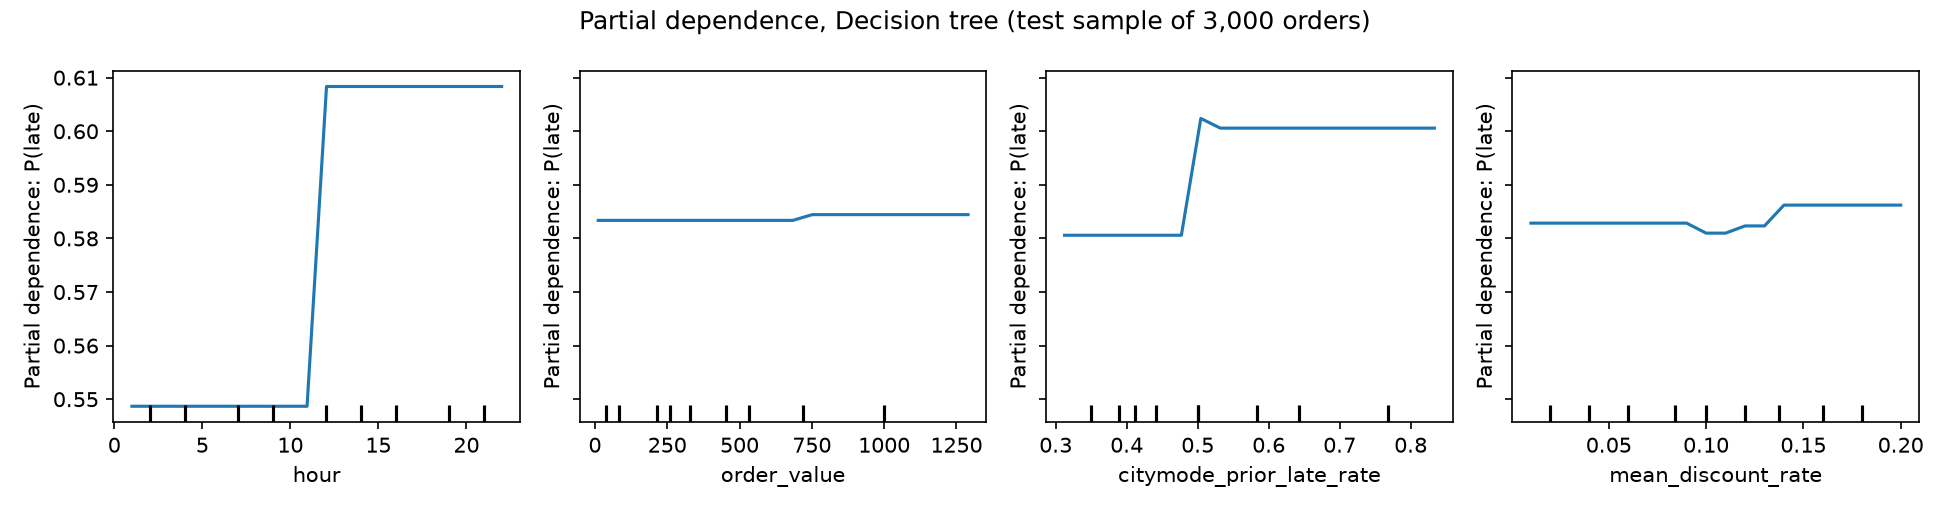
\includegraphics[width=\linewidth]{08_partial_dependence}
  \caption{Partial dependence of the predicted late probability, decision tree, on a test sample of 3{,}000 orders.}
  \label{fig:pdp}
\end{figure}

\begin{table}[H]
  \centering
  \caption{Drift check: the test period split at 2017-10-01. Saving is in USD per order under the expected-value policy.}
  \label{tab:drift}
  \footnotesize
  \begin{tabular}{l l r r c c c}
    \toprule
    \textbf{Period} & \textbf{Method} & \textbf{Orders} & \textbf{Median} & \textbf{PR-AUC} & \textbf{ROC-AUC} & \textbf{Saving/order} \\
    \midrule
    2017-07..09 & Decision tree & 5{,}028 & \usd{610} & 0.860 & 0.778 & 9.77 \\
                       & Lookup table  &         &           & 0.859 & 0.779 & 9.78 \\
                       & Rule B        &         &           & 0.814 & 0.753 & 7.28 \\
    2017-10..2018-01 & Decision tree & 8{,}043 & \usd{253} & 0.862 & 0.782 & 2.99 \\
                       & Lookup table  &         &           & 0.859 & 0.776 & 3.00 \\
                       & Rule B        &         &           & 0.813 & 0.749 & 1.16 \\
    \bottomrule
  \end{tabular}
\end{table}

\section{Reproducibility and code excerpts}
\label{app:code}

The code runs from a clean start and reproduces every number in this report. We checked this
by rebuilding it in a fresh virtual environment and comparing all 24 output tables. Repository:
\url{https://github.com/KenKout/ME3297_Project}. The raw dataset is not included in the
submission; \tcode{get\_data.py} extracts it from the Mendeley archive.

\begin{code}{bash}
python -m venv .venv && source .venv/bin/activate
pip install -r requirements.txt        # numpy 2.5.3, pandas 3.0.6, scikit-learn 1.9.1, matplotlib 3.11.2
python get_data.py path/to/8gx2fvg2k6-5.zip
python run_all.py                      # ~4 min; writes outputs/tables/*.csv and outputs/figures/*.png
\end{code}

\paragraph{Leakage-safe history features} (\tcode{\_prior\_history} in \tcode{src/data\_prep.py},
body only; comments in the code are in Vietnamese). For each order, it counts the earlier orders
of the same group whose outcome was already available (\tcode{avail} = order date + real
transit days + 1 day) at the current order time, and how many of those were late.

\inputcode[firstline=199,lastline=215]{python}{../src/data_prep.py}

The expected-value flagging rule (\Cref{eq:ev}) is a single line in \tcode{ev\_flag} in
\tcode{src/modeling.py}:

\begin{code}{python}
return np.asarray(p) * cost.effectiveness * cost.miss_fraction * np.asarray(value) > cost.action_cost
\end{code}

\section{Declaration of AI assistant use}
\label{app:ai}

As §9 of the project brief requires, we declare that an AI coding assistant (Kiro) was used
substantially in this project. It was used to:
\begin{itemize}
  \item draft the project proposal from the brief;
  \item write the analysis code (\tcode{get\_data.py}, \tcode{src/}, \tcode{run\_all.py}), including
        the data audit that uncovered the deterministic delivery patterns, and add explanatory
        comments in Vietnamese;
  \item run the pipeline, check that it reproduces from a clean environment, and draft this
        report in \LaTeX{} from the generated tables and figures.
\end{itemize}
\textbf{[Team to complete before submission: state what the team itself did. For example,
which analysis decisions you reviewed or changed, which numbers you re-checked against
\tcode{outputs/tables/}, and which sections you rewrote in your own words.]}

Every member has read the code and the report and is prepared to explain any line or
sentence of it during the presentations.


\end{document}
